\subsection{Topology Types}
Topologies are further classified as either regular or irregular ({\bf
  \cgrid{}} and {\bf \ugrid} respectively in \sciwms{} terminology)
which admit different data structures and algorithms for storage and
processing.

{\bf \cgrid{}} topologies refer geo-referenced locations and
geometries that can be defined analytically, e.g., rectilinear or
curvilinear grids. Storing \cgrid{} topologies amount to storing the
closed form formula. Algorithms for processing \cgrid{}s such as
finding nearest neighbors or finding points that fall withing a
polygonal subset are computed directly using the implicit \cgrid{}
representation.

{\bf \ugrid{}} are defined as topologies that are not regular, i.e.,
do not admit a closed form representation. \ugrid{} topologies offer
the highest level of flexibility from a visualization and modeling
standpoint as a higher sampling frequency may be used regions of
interest and less samples allocated for low-impact areas. For example,
figure~\ref{fig:usf_fvcom_ugrid} shows a \ugrid{} 2D topology used by
a climatological model for simulating hurricane conditions in the Gulf
of Mexico. Vertices represent location where values are estimated and
the connectivity defines an interpolation scheme, for the modeling and
visualization algorithms. The \ugrid{} topology allows the modelers to
save storage and computational resources by sparsely modeling areas
which are likewise sparsely populated, such as the center of the Gulf
while the Florida and Louisiana coastline have a very high spatial
sampling frequency allowing for higher model accuracy. However,
\ugrid{} topologies require explicit enumeration of verticies and
connectivity, and as such, require spatially-aware data structures for
optimal storage and processing.

Any NCML file which exposes the topology of an externally hosted
dataset according to the \cfugrid{} sepcification can be processed by
\sciwms{}. According the \cfugrid{} standard, the coordinates of
vertices in exposed as a list in the model's ambient space. For
example figure~\ref{fig:xytable} visualizes a list of a topology's
vertex locations as an array of coordinates in the real plane. Topolgy
connectivity is specified by a list of indicies into the vertex array
interpreted anticlockwise. Figure~\ref{fig:vtable} visualizes a 2D
connectivity list for the vertex array in figure~\ref{fig:xytable}
where each entry is an indexes an element of the vertex list:
$v_n^{\cdot}\in \{0,\ldots,N-1\}$. The rows specify triangles in an
anticlockwise manner. Triangle $m$ is specified by linking the
coordinates associated with vertex lists by connecting $v^0_m$ to
$v^1_m$ to $v^2_m$ and back to $v^0_m$.

\begin{figure}
  \centering
  \begin{subfigure}[t]{0.33\textwidth}
    \centering
    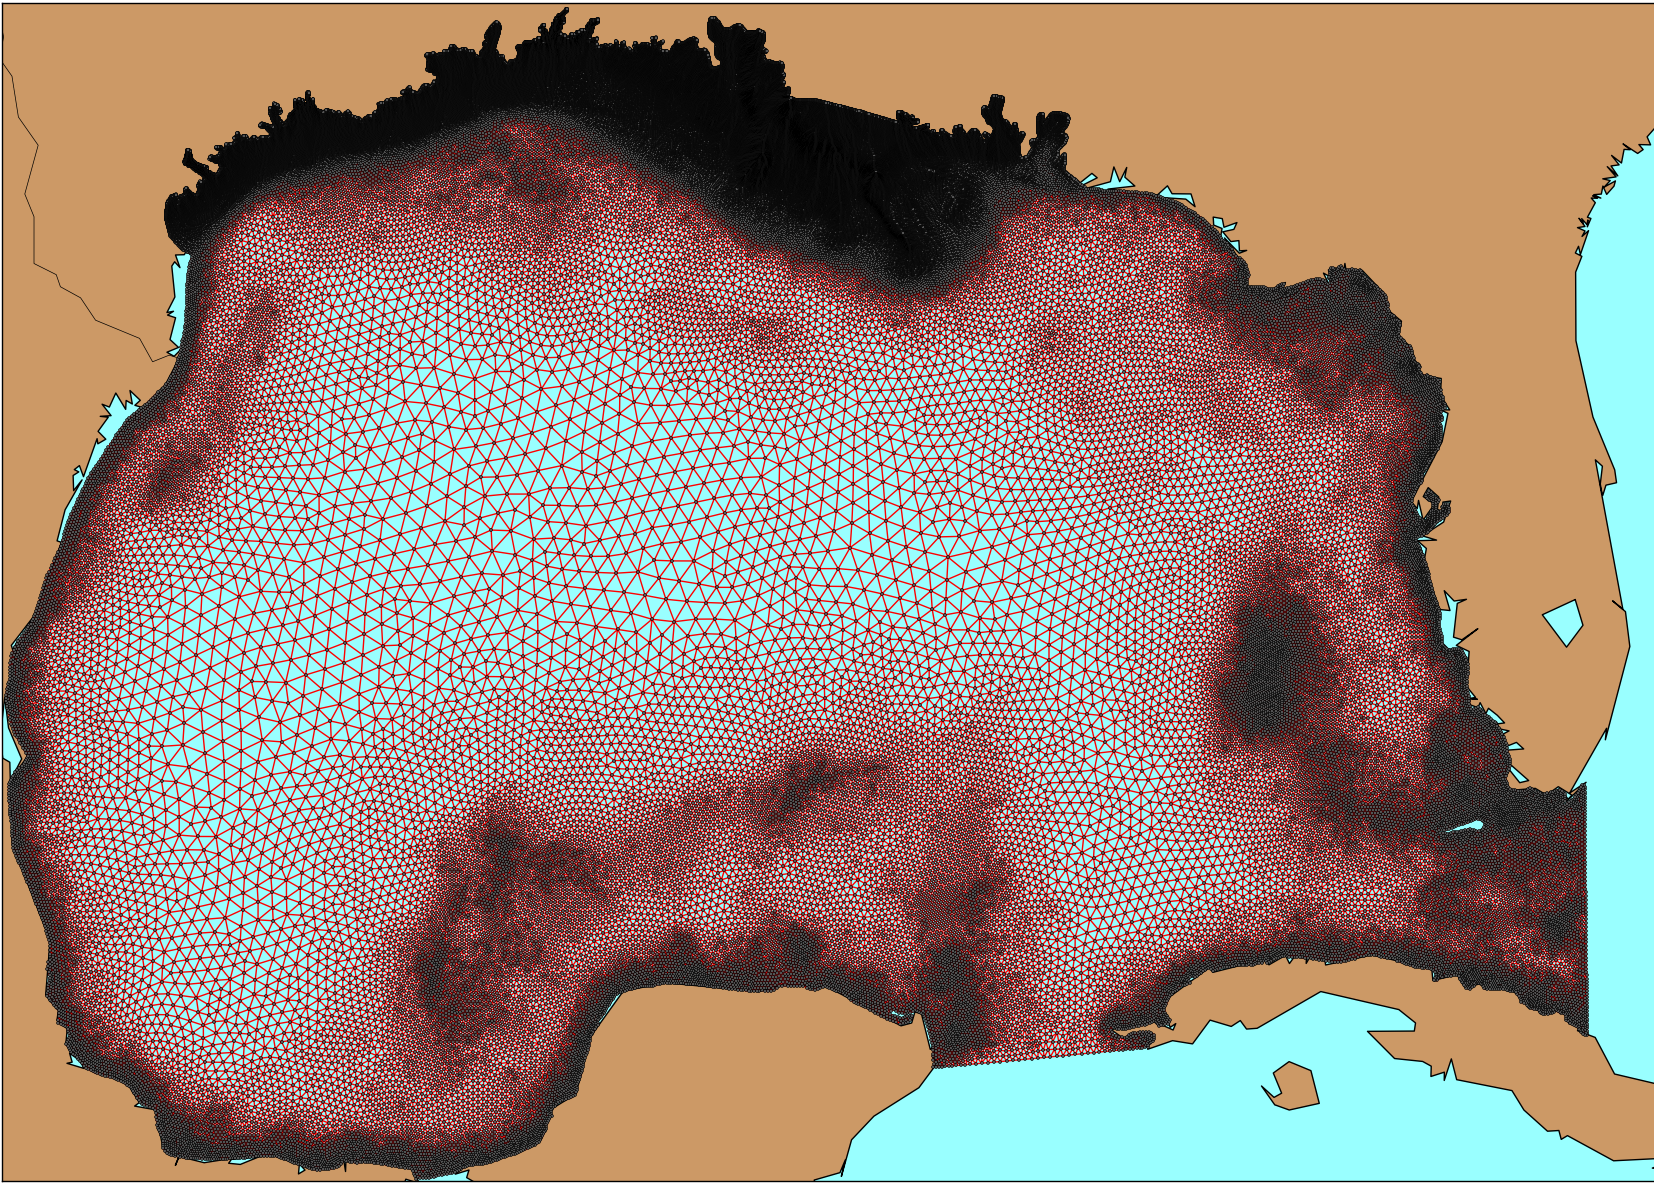
\includegraphics[height=1.3in]{../figs/USF_FVCOM_Hurricane_Ike_2D_final_run_with_waves_topology.png}
    \caption{}
    \label{fig:usf_fvcom_ugrid}
  \end{subfigure}
  \begin{subfigure}[t]{0.32\textwidth}
    \centering
    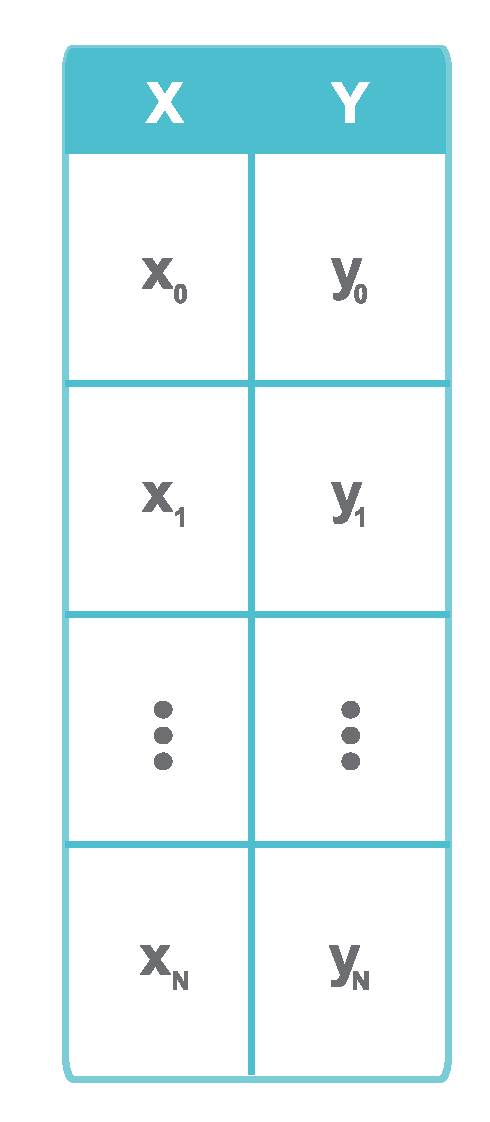
\includegraphics[height=1.35in]{../figs/xy_table}
    \caption{}
    \label{fig:xytable}
  \end{subfigure}
  \begin{subfigure}[t]{0.32\textwidth}
    \centering
    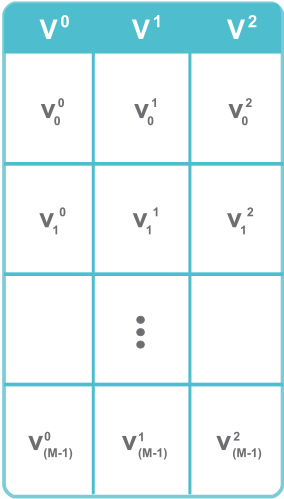
\includegraphics[height=1.35in]{../figs/v_table}
    \caption{}
    \label{fig:vtable}
  \end{subfigure}
  \caption{Unstructured grid location and connectivity arrays as
    specified by \cfugrid{} conventions. In this example, table (a)
    defines the location of 2D vertices: while (b) defines a 2D
    topology: a list of indicies on each row of verticies which
    specify a triangle. In this example, there are $N$ points and $M$
    triangles.}
\end{figure}
